\section{Quantitative Analysis}

\subsection{Combining the facets Contribution, SLA Usage and Data Integration Description}

\begin{figure}[h!]
\centering
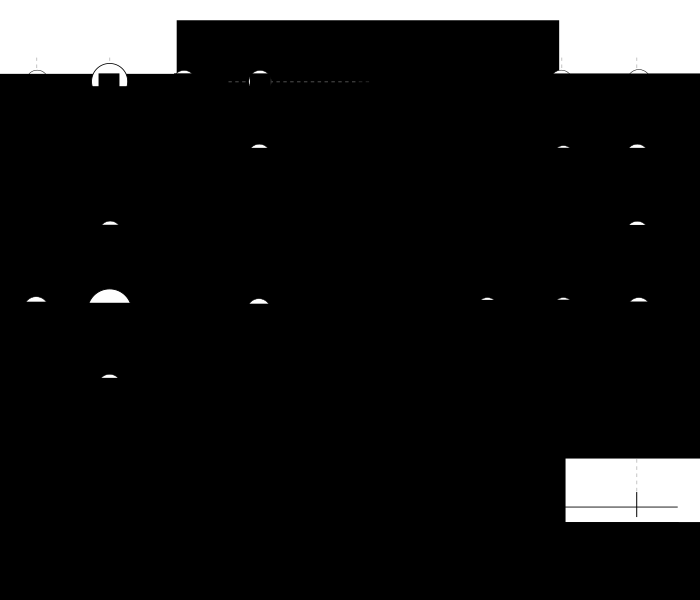
\includegraphics[scale=0.5]{figs/bubble-charts/Contribution-SLA-DIdescription.pdf} 
\caption{...}
\end{figure}

\subsection{Combining the facets Data Integration Environment, Contribution and Research}

\begin{figure}[h!]
\centering
\includegraphics[scale=0.5]{figs/bubble-charts/DI-Environment-Contribution-Research.pdf}
\caption{...}
\end{figure}

\subsection{Combining the facets SLA Usage and Contribution}

\begin{figure}[h!]
\centering
\includegraphics[scale=0.7]{figs/bubble-charts/SLA-Contribution.pdf}
\caption{...}
\end{figure}


\subsection{Combining the facets Data Quality, Data Integration Environment and Data Integration Description}

Combining the facet Data Quality with the facets Data Integration Environment e Data Integration Description
(Figure~\ref{fig:facet4}) it is possible to note which quality of service parameters have been applied in
data integration studies.
It is also possible to identify which are the most applied data integration environment and description.
First of all, ...

\begin{figure}[h!]
\centering
\includegraphics[scale=0.53]{figs/bubble-charts/Data-Quality-DI.pdf}
\caption{Facets Data Quality, Data Integration Environment and Data Integration Description}\label{fig:facet4}
\end{figure}
